%% Cyberinfrastructure Shell (CIShell) Core Specification
%%
%% Copyright 2006,2007,2008 Indiana University
%%
%% Licensed under the Apache License, Version 2.0 (the "License");
%% you may not use this file except in compliance with the License.
%% You may obtain a copy of the License at
%%
%%     http://www.apache.org/licenses/LICENSE-2.0
%%
%% Unless required by applicable law or agreed to in writing, software
%% distributed under the License is distributed on an "AS IS" BASIS,
%% WITHOUT WARRANTIES OR CONDITIONS OF ANY KIND, either express or implied.
%% See the License for the specific language governing permissions and
%% limitations under the License.
%%
%

\chapter{Framework API}

\section*{\textit{Version 1.0}}

\section{Introduction}

The \class{org.cishell.framework} package and subpackages define the core of
CIShell. The key components being algorithms, data, and CIShell service access.

\subsection{Entities}

\begin{itemize}
  \item \textit{AlgorithmFactory} - The service interface for algorithms.
  A factory class which creates an \class{Algorithm} for execution from input
  data.
  \item \textit{Algorithm} - The interface for the code execution part of the
  algorithm.
  \item \textit{AlgorithmProperty} - The interface which provides string
  constants for an algorithm's service metadata.
  \item \textit{ParameterMutator} - The interface an \class{AlgorithmFactory}
  extends to provide the ability to add, remove, or modify its input
  parameters specification (see section \ref{GUISpec}) before being transformed
  into a form for user input.
  \item \textit{DataValidator} - The interface an \class{AlgorithmFactory}
  extends to provide additional data validation in addition to the data format validation
  that an application should provide ahead of time.
  \item \textit{ProgressTrackable} - The interface an \class{Algorithm} extends
  to allow for more detailed monitoring and control of an \class{Algorithm}'s
  progress while executing.
  \item \textit{ProgressMonitor} - The interface for a class to be passed in to
  a \class{ProgressTrackable} \class{Algorithm} so that the \class{Algorithm}
  can be controlled and provide information on its progress while executing.
  \item \textit{Data} - The interface used to pass data (other than
  input parameters) and its metadata between algorithms.
  \item \textit{BasicData} - A simple implementation of the \class{Data}
  interface.
  \item \textit{DataProperty} - The interface which provides string constants
  for \class{Data} metadata.
  \item \textit{CIShellContext} - The interface for a class to be passed in to
  an \class{AlgorithmFactory} for use in gaining access to standard CIShell
  services.
  \item \textit{LocalCIShellContext} - A simple implementation of the
  \class{CIShellContext} interface which pulls CIShell services from the OSGi
  service registry.
\end{itemize}

\begin{figure}[htb!]
\centering
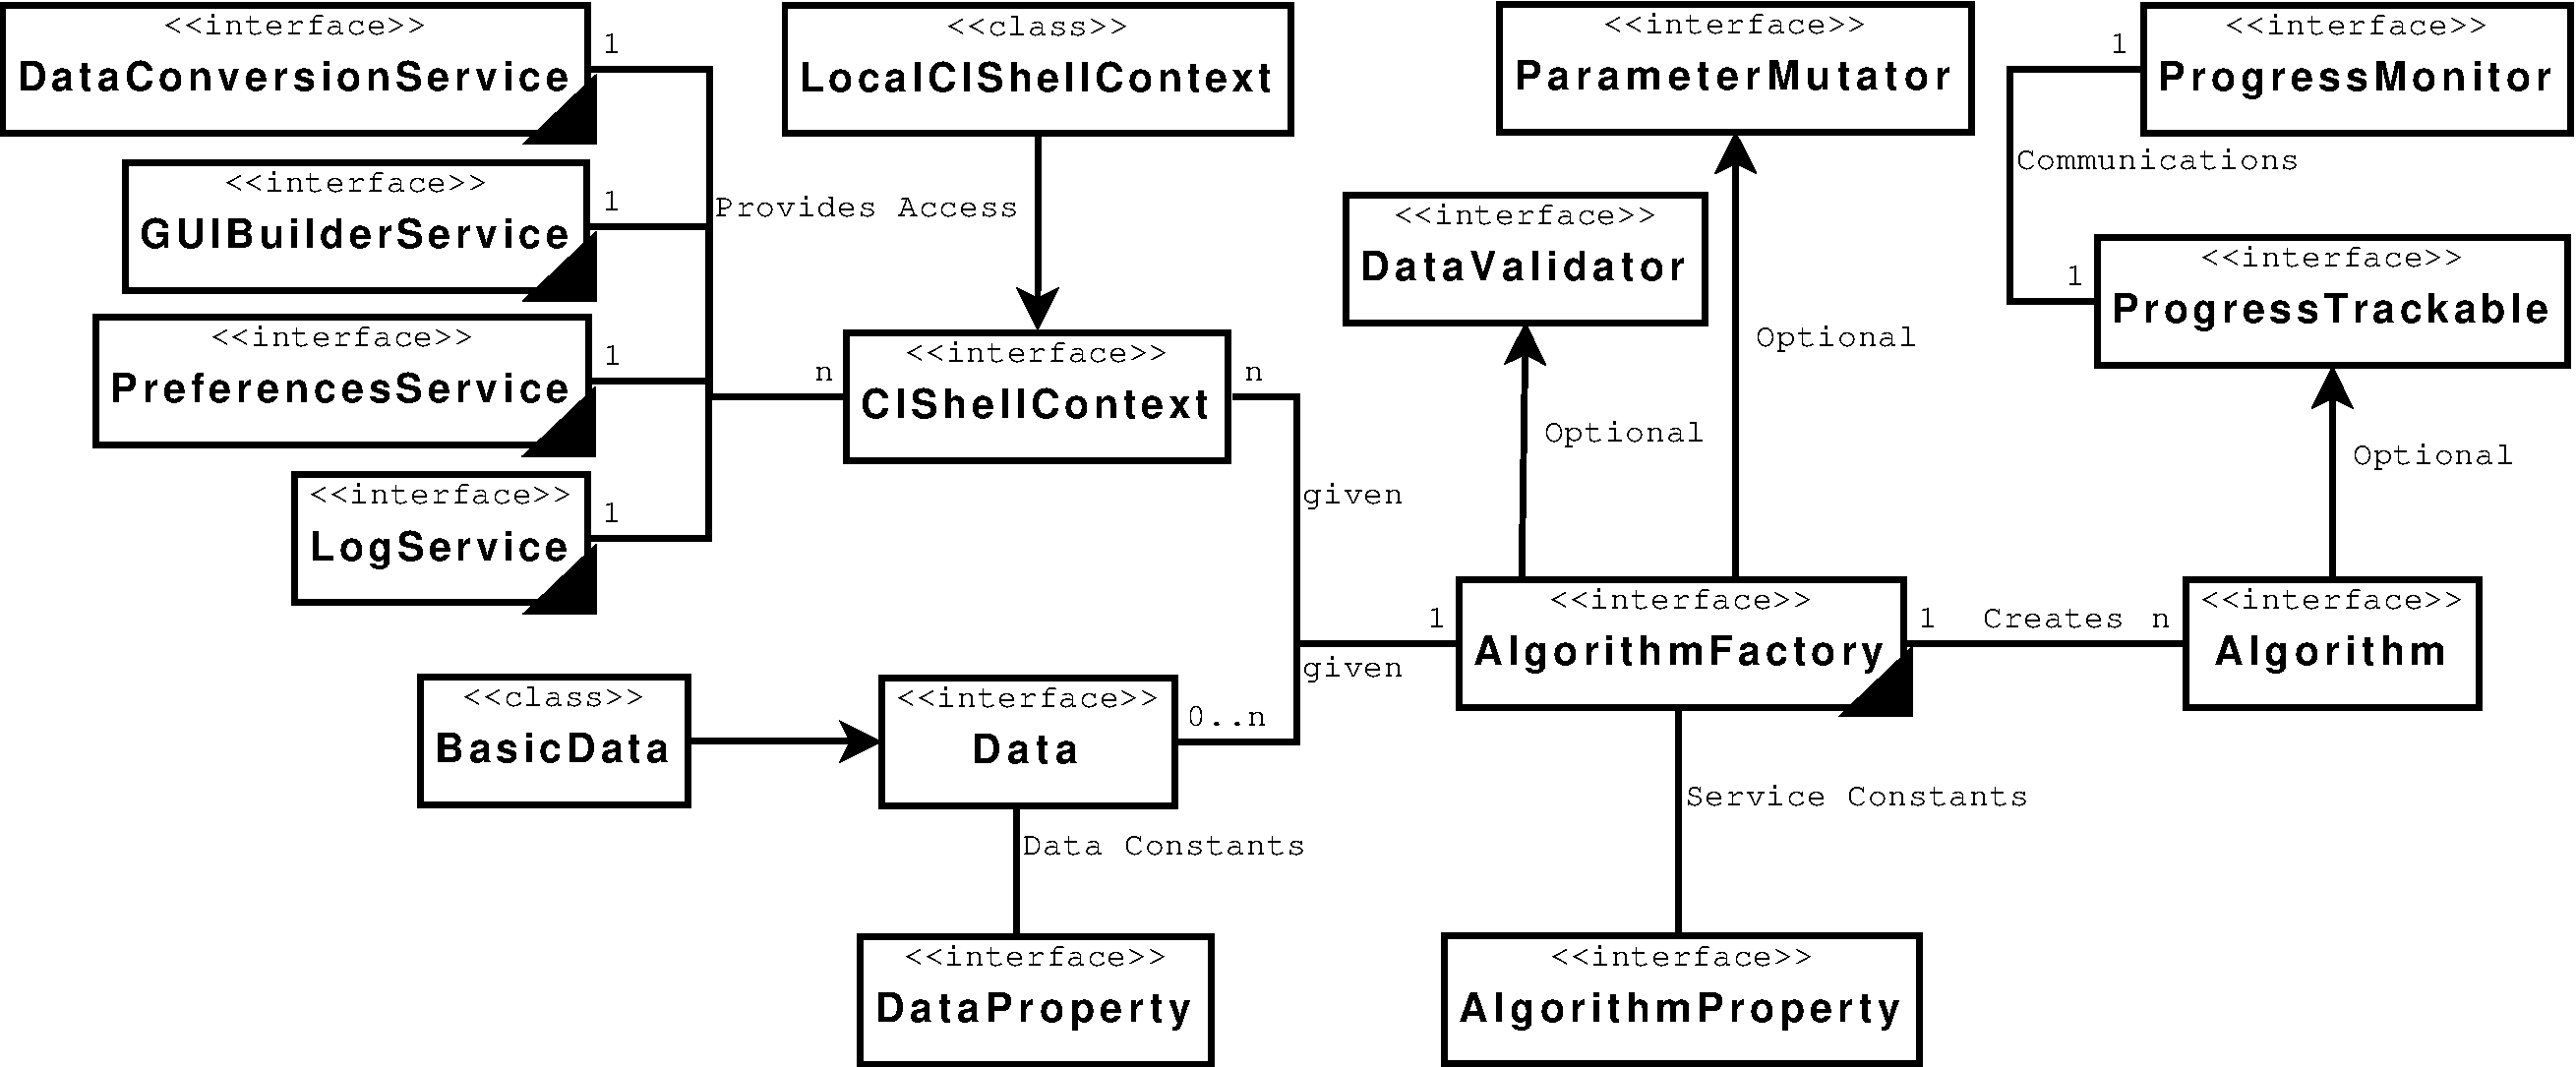
\includegraphics[width=150mm]{../img/cishellInteraction.pdf}
\caption{org.cishell.framework Class Diagram}
\label{fig:cishellInteraction}
\end{figure}

\subsection{Operations}

The algorithm developer should implement algorithms as described in this
specification. The system developer will provide the services required by CIShell
in OSGi's service registry. Application developers will provide everything else,
orchestrating the passing of information between algorithms.
